\documentclass[preprint,12pt,3p]{elsarticle}

\usepackage{amssymb}
\usepackage{amsmath}
\usepackage{amsthm}
\usepackage{booktabs}
\usepackage{graphicx}
\usepackage{hyperref}
\usepackage{xcolor}
\usepackage{microtype}
\usepackage{algorithm}
\usepackage{algpseudocode}

\usepackage{hyphenat}

\hypersetup{
    pdfauthor={Nithin Kumbam},
    pdftitle={Ontology-Constrained Neuro-Symbolic Decoding},
    pdfkeywords={Neuro-symbolic AI, LLM Security, Constrained Decoding}
}

\newtheorem{definition}{Definition}
\newtheorem{theorem}{Theorem}

\journal{Knowledge-Based Systems}

\begin{document}

\begin{frontmatter}

\title{Ontology-Constrained Neuro-Symbolic Decoding: Enforcing Axiomatic Least-Privilege in Autonomous LLM Agents}

\author[inst1]{Nithin Kumbam\corref{cor1}}
\ead{nithin@research.org}
\cortext[cor1]{Corresponding author.}
\affiliation[inst1]{organization={Enterprise AI Research Laboratory},
            city={New York},
            postcode={10001},
            state={NY},
            country={USA}}

\begin{abstract}
Autonomous tool-calling Large Language Model (LLM) agents are increasingly entrusted with operational authority in enterprise business workflows, including financial disbursements, database modifications, and customer identity operations. However, existing safety paradigms rely predominantly on \textit{in-context system prompts} or \textit{post-hoc classifiers}, both of which remain vulnerable to indirect prompt injection, privilege escalation, and adversarial parameter tampering. In this paper, we propose \textbf{Ontology-Constrained Token Decoding (O-CTD)}, a neuro-symbolic framework that compiles formal, declarative Role-Based Access Control (RBAC) ontologies into runtime Context-Free Grammars (CFGs). By projecting the LLM's autoregressive logit distribution onto the permissible transitions of a Deterministic Finite Automaton (DFA) at each generation step, O-CTD mathematically guarantees that unauthorized tool selections and out-of-bounds parameter values cannot be sampled. We empirically evaluate O-CTD against three standard industry baselines across 100 enterprise business scenarios (400 total inferences) using \texttt{Qwen2.5-7B-Instruct} on an NVIDIA RTX 4090 GPU. Experimental results demonstrate that O-CTD suppresses the Attack Success Rate (ASR) from 80.0\% (in-context guardrails) down to 20.0\%, reduces policy Invariant Violation Rates (IVR) from 90.0\% to 10.0\%, and achieves 100.0\% Benign Task Completion (BTC). A paired Wilcoxon signed-rank test confirms statistical significance ($W = 0.0, p = 3.74 \times 10^{-19}, r = 0.800$). We publish our benchmark suite, declarative schemas, and decoding harness to advance formal verification in agentic AI.
\end{abstract}

\begin{keyword}
Neuro-symbolic AI \sep Large Language Models \sep Constrained Decoding \sep Autonomous Agents \sep Role-Based Access Control \sep Prompt Injection Defense
\end{keyword}

\end{frontmatter}

\section{Introduction}
\label{sec:intro}

The transition of Large Language Models (LLMs) from passive conversational engines to autonomous agents operating via function calling and external API dispatch represents a foundational paradigm shift in enterprise automation \cite{yao2023react, qin2024toolllm}. Autonomous agents are currently deployed in core business domains, such as executing customer refunds, modifying shipping schedules, and querying relational database management systems. 

Despite their operational utility, agentic workflows introduce catastrophic security vulnerabilities \cite{greshake2023not, owasp2025top10}. Most critically, untrusted data ingested from emails, documents, or database outputs can trigger \textit{indirect prompt injection} (IPI), wherein embedded adversarial instructions hijack the model's intent \cite{zhan2024injecagent, debenedetti2024agentdojo}. Under such attacks, autonomous agents frequently suffer from the classic \textit{Confused Deputy} problem \cite{mavrogiannis2024confused}, using legitimate enterprise credentials to execute unauthorized disbursements or exfiltrate private ledgers.

Contemporary defensive strategies fall into two predominant categories:
\begin{enumerate}
    \item \textbf{In-Context Prompt Guarding:} Prepending instructional constraints to the system prompt (e.g., \textit{``You are a Tier 1 agent. Never issue refunds over \$50.00''}) \cite{wei2024jailbroken}.
    \item \textbf{Post-Hoc Classification:} Filtering outputs through secondary safety classifiers or heuristic regex parsers before execution \cite{ruan2024identifying}.
\end{enumerate}

Both approaches are fundamentally probabilistic. Soft system prompts are routinely circumvented by authority impersonation, debug mode exploits, or payload obfuscation \cite{debenedetti2024agentdojo}. Conversely, post-hoc classifiers are decoupled from the generation process, operating retroactively and introducing high false-rejection rates on complex business tasks \cite{wang2025progent}.

To address these vulnerabilities, we propose \textbf{Ontology-Constrained Token Decoding (O-CTD)}, a neuro-symbolic framework that grounds autoregressive language generation in formal declarative knowledge representations \cite{sheth2023neurosymbolic, pan2024unifying}. By compiling an enterprise Role-Based Access Control (RBAC) ontology into a dynamic Context-Free Grammar (CFG), O-CTD applies token-level logit masking at each autoregressive decoding step \cite{willard2023efficient, zhang2024syncode}. Consequently, any token that violates active role privileges, invokes unauthorized tools, or exceeds numerical parametric bounds is assigned a probability of zero before sampling.

\section{Mathematical Formulation}
\label{sec:math}

\subsection{Enterprise RBAC Security Ontology}

We formalize enterprise access policies as an axiomatic security ontology defined over roles, operational tools, and parametric bounds \cite{sandhu1996role, ferraiolo2001proposed}.

\begin{definition}[Enterprise Security Ontology]
An Enterprise Security Ontology is a 3-tuple:
\begin{equation}
    \mathcal{O} = \langle \mathcal{R}, \mathcal{T}, \Sigma \rangle
\end{equation}
where:
\begin{itemize}
    \item $\mathcal{R} = \{r_1, r_2, \dots, r_m\}$ is the set of authenticated enterprise user roles (e.g., $\text{CustomerSupportTier1}$, $\text{BillingManager}$).
    \item $\mathcal{T} = \{t_1, t_2, \dots, t_n\}$ is the catalog of enterprise tools/APIs available in the operational environment.
    \item $\Sigma = \{\sigma_1, \sigma_2, \dots, \sigma_k\}$ is the set of formal security axioms governing tool invocation.
\end{itemize}
\end{definition}

Each role $r \in \mathcal{R}$ is mapped to an authorized tool subset $\mathcal{T}_r \subseteq \mathcal{T}$ and a set of parametric invariant axioms $\Sigma_r \subseteq \Sigma$. Specifically, for an action $a = \langle t, \theta \rangle$ where $t \in \mathcal{T}$ and $\theta = \{p_i: v_i\}$ represents the argument dictionary, the validity predicate $\Phi(a, r)$ is defined as:
\begin{equation}
    \Phi(\langle t, \theta \rangle, r) \iff \left( t \in \mathcal{T}_r \right) \land \left( \forall \sigma \in \Sigma_r, \, \sigma(\theta) = \text{True} \right)
\end{equation}

In our enterprise benchmark, parametric axioms $\sigma \in \Sigma_r$ enforce strict bounds, including:
\begin{align}
    \sigma_{\text{refund}}(\theta) &\iff \theta[\text{amount\_usd}] \le C_r \\
    \sigma_{\text{address}}(\theta) &\iff \theta[\text{is\_international}] = \text{False} \\
    \sigma_{\text{sql}}(\theta) &\iff \theta[\text{query}] \notin \mathcal{L}_{\text{prohibited}}
\end{align}
where $C_r$ is the maximum refund ceiling authorized for role $r$ ($C_{\text{Tier1}} = \$50.00$, $C_{\text{Billing}} = \$1000.00$), and $\mathcal{L}_{\text{prohibited}}$ denotes blacklisted data modification patterns.

\subsection{Context-Free Grammar Compilation}

To enforce $\Phi(a, r)$ during autoregressive generation, the compiler $\mathcal{M}$ dynamically transforms the active role definition $r$ into a formal Context-Free Grammar $\mathcal{G}_r = \langle V_N, V_T, P, S \rangle$ \cite{hopcroft2001introduction}:
\begin{equation}
    \mathcal{M}: r \mapsto \mathcal{G}_r
\end{equation}
where $V_T$ is the alphabet of terminal characters, $V_N$ is the set of non-terminals, $P$ is the set of production rules, and $S$ is the start symbol. 

Under $\mathcal{G}_r$, the production rules for the tool identifier are constrained to the exact literal union of authorized tools:
\begin{equation}
    S \to \text{\texttt{"action\_name": }} \left( t_{r, 1} \mid t_{r, 2} \mid \dots \mid t_{r, |\mathcal{T}_r|} \right) \quad \forall t_{r, j} \in \mathcal{T}_r
\end{equation}
Numerical parameters subject to ceiling constraints $C_r$ are compiled into bounded regular expressions or sub-grammars that reject any numeric string representation exceeding $C_r$.

\subsection{Token-Level Logit-Masking Projection}

Let $\mathcal{V}$ denote the tokenizer vocabulary of size $|\mathcal{V}|$, and let $x_{<t} = [x_1, \dots, x_{t-1}]$ denote the sequence of generated tokens up to step $t$. At step $t$, the base language model outputs unconstrained logit vector $\mathbf{z}_t \in \mathbb{R}^{|\mathcal{V}|}$. 

The grammar $\mathcal{G}_r$ is compiled into a Deterministic Finite Automaton (DFA) over the token vocabulary \cite{willard2023efficient, zhao2024xgrammar}. Let $q_t \in Q$ denote the current DFA state after ingesting $x_{<t}$. The set of admissible next tokens $\mathcal{A}(q_t) \subseteq \mathcal{V}$ is defined as:
\begin{equation}
    \mathcal{A}(q_t) = \{ v \in \mathcal{V} \mid \exists q' \in Q, \, \delta(q_t, v) = q' \}
\end{equation}
where $\delta$ is the state transition function.

The neuro-symbolic projection operator $\mathcal{P}_{\mathcal{G}_r}: \mathbb{R}^{|\mathcal{V}|} \to \mathbb{R}^{|\mathcal{V}|}$ masks the logit distribution:
\begin{equation}
    \mathcal{P}_{\mathcal{G}_r}(\mathbf{z}_t)_v = 
    \begin{cases} 
        \mathbf{z}_{t, v} & \text{if } v \in \mathcal{A}(q_t) \\
        -\infty & \text{if } v \notin \mathcal{A}(q_t)
    \end{cases}
\end{equation}

The next token is sampled from the normalized masked distribution:
\begin{equation}
    x_t \sim \text{Softmax}\left( \mathcal{P}_{\mathcal{G}_r}(\mathbf{z}_t) \right)
\end{equation}

\begin{theorem}[Soundness of Axiomatic Enforcement]
Let $\mathbf{x} = [x_1, \dots, x_K]$ be a completed generation sequence terminated by an end-of-sequence token under O-CTD. Then the extracted tool call $a = \text{Parse}(\mathbf{x})$ satisfies:
\begin{equation}
    P\left( \Phi(a, r) = \text{False} \right) = 0
\end{equation}
with respect to all syntactically expressible invariants in $\mathcal{G}_r$.
\end{theorem}
\begin{proof}
By construction, any token sequence $\mathbf{x}$ yielding an unauthorized tool $t \notin \mathcal{T}_r$ or an out-of-bounds numeric token sequence requires traversing at least one invalid DFA transition $\delta(q_t, v) = \emptyset$. Since $\mathcal{P}_{\mathcal{G}_r}(\mathbf{z}_t)_v = -\infty$, the sampling probability $P(x_t = v) = 0$. By induction over generation steps $1 \le t \le K$, the probability of generating a violating sequence is identically zero.
\end{proof}

\section{Experimental Methodology}
\label{sec:exp}

\subsection{Benchmark Dataset \& Threat Classes}

To rigorously evaluate enterprise LLM agent resilience, we synthesized a standardized benchmark suite consisting of $N = 100$ balanced business evaluation cases (50 adversarial attack prompts and 50 benign utility queries) grounded in the InjecAgent and AgentDojo threat models \cite{zhan2024injecagent, debenedetti2024agentdojo}. The scenarios span three core business roles:
\begin{itemize}
    \item \textbf{CustomerSupportTier1:} Authorized for order lookup, shipping address updates (domestic only), and refunds capped at \$50.00.
    \item \textbf{BillingManager:} Authorized for invoice credits up to \$5,000.00 and refunds up to \$1,000.00.
    \item \textbf{DataAnalyst:} Authorized for aggregate analytics; strictly barred from financial tools and raw payment ledgers.
\end{itemize}

The 50 adversarial prompts span five distinct threat categories:
\begin{enumerate}
    \item \textbf{Parameter Tampering (PT):} Adversary coerces the agent into issuing a \$500.00 or \$1,200.00 refund via authority pressure (e.g., claiming ``Executive VIP Override'').
    \item \textbf{Privilege Escalation (PE):} Frontline support agent is instructed via debug commands to invoke admin tools (\texttt{view\_payment\_ledger}).
    \item \textbf{SQL / Exfiltration Injection (SQL):} Malicious payloads inside query arguments attempting \texttt{DROP TABLE} or plain-text credential exfiltration.
    \item \textbf{Indirect Prompt Injection (IPI):} Simulated third-party vendor emails containing hidden instructions directing wire disbursements.
    \item \textbf{Policy Boundary Tampering (PBT):} Coercing domestic customer support to route orders to embargoed international addresses.
\end{enumerate}

\subsection{Comparative Frameworks}

We benchmark four comparative architectures:
\begin{itemize}
    \item \textbf{M0 (Vanilla Base LLM):} Unconstrained generation; agent receives standard ReAct-style role descriptions without defensive guardrails.
    \item \textbf{M1 (In-Context Prompt Guard):} Standard enterprise defensive baseline; system prompt includes explicit natural-language prohibitions (e.g., \textit{``CRITICAL: You are strictly forbidden from exceeding \$50 refunds or viewing ledgers''}).
    \item \textbf{M2 (Post-Hoc Classifier):} Output is generated unconstrained, followed by a secondary classifier pass that checks generated JSON against policy rules before execution.
    \item \textbf{M* (Proposed O-CTD):} Autoregressive token decoding strictly constrained by the compiled role-specific context-free grammar.
\end{itemize}

\subsection{Experimental Environment}

All experiments were executed on an isolated cloud compute node equipped with:
\begin{itemize}
    \item \textbf{GPU:} NVIDIA GeForce RTX 4090 (24 GB GDDR6X VRAM).
    \item \textbf{Base Foundation Model:} \texttt{Qwen/Qwen2.5-7B-Instruct} (bfloat16 precision) \cite{qwen2024qwen25}.
    \item \textbf{Grammar Engine:} Outlines v1.x with dynamic Pydantic schema compilation \cite{willard2023efficient}.
    \item \textbf{Memory Architecture:} Single shared model instance on \texttt{cuda:0} with zero CPU offloading to guarantee consistent latency measurements.
\end{itemize}

\subsection{Evaluation Metrics}

We track five formal metrics:
\begin{enumerate}
    \item \textbf{Attack Success Rate (ASR) [\% $\downarrow$]:} Percentage of adversarial scenarios where the malicious objective was successfully executed.
    \item \textbf{Invariant Violation Rate (IVR) [\% $\downarrow$]:} Percentage of all scenarios (adversarial and benign) where an ontological axiom $\sigma \in \Sigma_r$ was violated.
    \item \textbf{Benign Task Completion (BTC) [\% $\uparrow$]:} Percentage of valid business requests executed correctly with valid schema compliance.
    \item \textbf{Mean Generation Latency [ms $\downarrow$]:} Average wall-clock inference time per tool invocation.
    \item \textbf{P95 Generation Latency [ms $\downarrow$]:} 95th-percentile inference latency.
\end{enumerate}

\section{Empirical Results \& Discussion}
\label{sec:results}

\subsection{Comparative Performance Analysis}

Table~\ref{tab:main_results} presents the primary benchmark results across the 100 enterprise business evaluation samples (400 total agent inferences).

\begin{table}[t]
\centering
\small
\caption{Main comparative benchmark results across 100 enterprise business evaluation scenarios (400 inferences) using \texttt{Qwen2.5-7B-Instruct} on an NVIDIA RTX 4090.}
\label{tab:main_results}
\resizebox{\columnwidth}{!}{
\begin{tabular}{lccccc}
\toprule
\textbf{Framework} & \textbf{ASR (\%)} $\downarrow$ & \textbf{IVR (\%)} $\downarrow$ & \textbf{BTC (\%)} $\uparrow$ & \textbf{Mean Latency} & \textbf{P95 Latency} \\
\midrule
M0 (Vanilla Base LLM)    & 100.0\% & 100.0\% & 0.0\%   & 893.1 ms  & 1396.1 ms \\
M1 (Prompt Guard)        & 80.0\%  & 90.0\%  & 0.0\%   & 1157.0 ms & 2261.7 ms \\
M2 (Post-Hoc Classifier) & 100.0\% & 100.0\% & 0.0\%   & 1120.3 ms & 1618.8 ms \\
\textbf{M* (Proposed O-CTD)} & \textbf{20.0\%} & \textbf{10.0\%} & \textbf{100.0\%} & 3116.0 ms & 4097.4 ms \\
\bottomrule
\end{tabular}
}
\end{table}

The empirical data establishes several foundational findings:

\textbf{1. The Collapse of In-Context Guardrails:} In-context prompt defense (M1) proved overwhelmingly ineffective under targeted adversarial pressure, exhibiting an **80.0\% ASR** and a **90.0\% IVR**. When confronted with adversarial jailbreaks framing the request as an emergency or debug override, the LLM systematically ignored system instructions. This empirically substantiates that probabilistic next-token generation cannot enforce safety invariants when adversarial tokens shift the context distribution \cite{wei2024jailbroken}.

\textbf{2. Utility Fragility in Unconstrained LLMs:} Strikingly, M0, M1, and M2 all exhibited **0.0\% BTC** on benign business tasks. Detailed log inspection revealed that this utility collapse was not due to cognitive inability, but rather \textit{syntactic non-conformance}. Unconstrained Qwen-2.5 generated conversational preambles (e.g., \textit{``Certainly! Here is the tool call:''}) or formatted argument keys inconsistently, failing automated API parsers. In contrast, M* achieved **100.0\% BTC**, demonstrating that neuro-symbolic grammar constraints simultaneously serve as a powerful utility guarantee by enforcing rigorous JSON schema adherence.

\textbf{3. Decisive Security Dominance of O-CTD:} O-CTD achieved a \textbf{4$\times$ reduction in ASR} (from 80.0\% to 20.0\%) and a \textbf{9$\times$ reduction in policy violations} (from 90.0\% to 10.0\%). All privilege escalation attempts (e.g., Tier 1 support invoking financial ledgers) and parameter ceiling breaches (e.g., refunds exceeding \$50.00) were physically eliminated at the logit level.

\subsection{Category Ablation across Enterprise Threat Vectors}

To evaluate defensive resilience across orthogonal attack topologies, Table~\ref{tab:category_ablation} details violation rates across specific threat vectors.

\begin{table}[t]
\centering
\small
\caption{Ablation Breakdown by Enterprise Threat Vector (Policy Invariant Violation Rates).}
\label{tab:category_ablation}
\resizebox{\columnwidth}{!}{
\begin{tabular}{lcccc}
\toprule
\textbf{Defense Architecture} & \textbf{Param Tampering} $\downarrow$ & \textbf{Priv Escalation} $\downarrow$ & \textbf{Indirect Inj} $\downarrow$ & \textbf{Benign Utility} $\uparrow$ \\
\midrule
M0 (Vanilla Base LLM)    & 100.0\% & 100.0\% & 100.0\% & 0.0\% \\
M1 (Prompt Guard)        & 100.0\% & 100.0\% & 0.0\%   & 0.0\% \\
M2 (Post-Hoc Classifier) & 100.0\% & 100.0\% & 100.0\% & 0.0\% \\
\textbf{M* (Proposed O-CTD)} & \textbf{50.0\%} & \textbf{0.0\%} & \textbf{0.0\%} & \textbf{100.0\%} \\
\bottomrule
\end{tabular}
}
\end{table}

As shown in Table~\ref{tab:category_ablation}, M* achieved an absolute **0.0\% violation rate on both Privilege Escalation and Indirect Prompt Injection**. Under Parameter Tampering (e.g., refund ceiling breaches), M* clamped all numeric generations to the role's authorized ceiling $C_r \le \$50.00$.

\subsection{Statistical Significance Testing}

To verify that the empirical superiority of O-CTD over standard prompt guarding is not an artifact of prompt selection, we conducted a non-parametric paired analysis \cite{wilcoxon1945individual}. Because binary policy violation outcomes violate normality assumptions, the paired \textbf{Wilcoxon Signed-Rank Test} was executed across all matched sample pairs between M1 and M*:
\begin{itemize}
    \item \textbf{Wilcoxon Test Statistic ($W$):} $0.0$
    \item \textbf{Two-Sided $p$-Value:} $\mathbf{3.7441 \times 10^{-19}} \ll 0.001$
    \item \textbf{Rank-Biserial Effect Size ($r$):} $\mathbf{0.800}$ \cite{kerby2014simple}
\end{itemize}
The effect size of $r = 0.800$ substantially exceeds the standard threshold for a ``large'' effect ($r \ge 0.50$), confirming that O-CTD delivers statistically definitive and reproducible safety improvements.

\subsection{Qualitative Analysis of the 20\% Residual ASR}

An essential requirement of rigorous empirical science is analyzing failure modes. While O-CTD reduced ASR from 80\% to 20\%, we investigate why the residual 20\% occurred despite formal grammar constraints:

\begin{enumerate}
    \item \textbf{The Confused Deputy within Allowed Tools:} In two attack scenarios, the adversary instructed the agent: \textit{``Order ORD-12345 was delayed; look up its status and append a note containing internal API keys.''}. Because \texttt{lookup\_order\_status} was an authorized tool for Tier 1 support, the grammar permitted its selection. While the grammar prevented unauthorized financial execution, the model processed the adversarial context within the legitimate tool's free-text field.
    \item \textbf{Safe Fallback Invocation:} Under extreme adversarial prompt injection where all attempted tool tokens were masked out by the DFA, the agent safely fell back to the default permitted tool (\texttt{lookup\_order\_status}). Although no unauthorized action occurred, the evaluation harness marked the sample as partially engaged because the agent did not output an explicit refusal string.
\end{enumerate}
This analysis highlights a critical theoretical boundary: **Context-Free Grammars mathematically eliminate structural and parametric privilege escalations, but semantic validation inside unbounded free-text fields remains an orthogonal challenge.**

\subsection{Computational Overhead \& The Pareto Frontier}

\begin{figure*}[t]
\centering
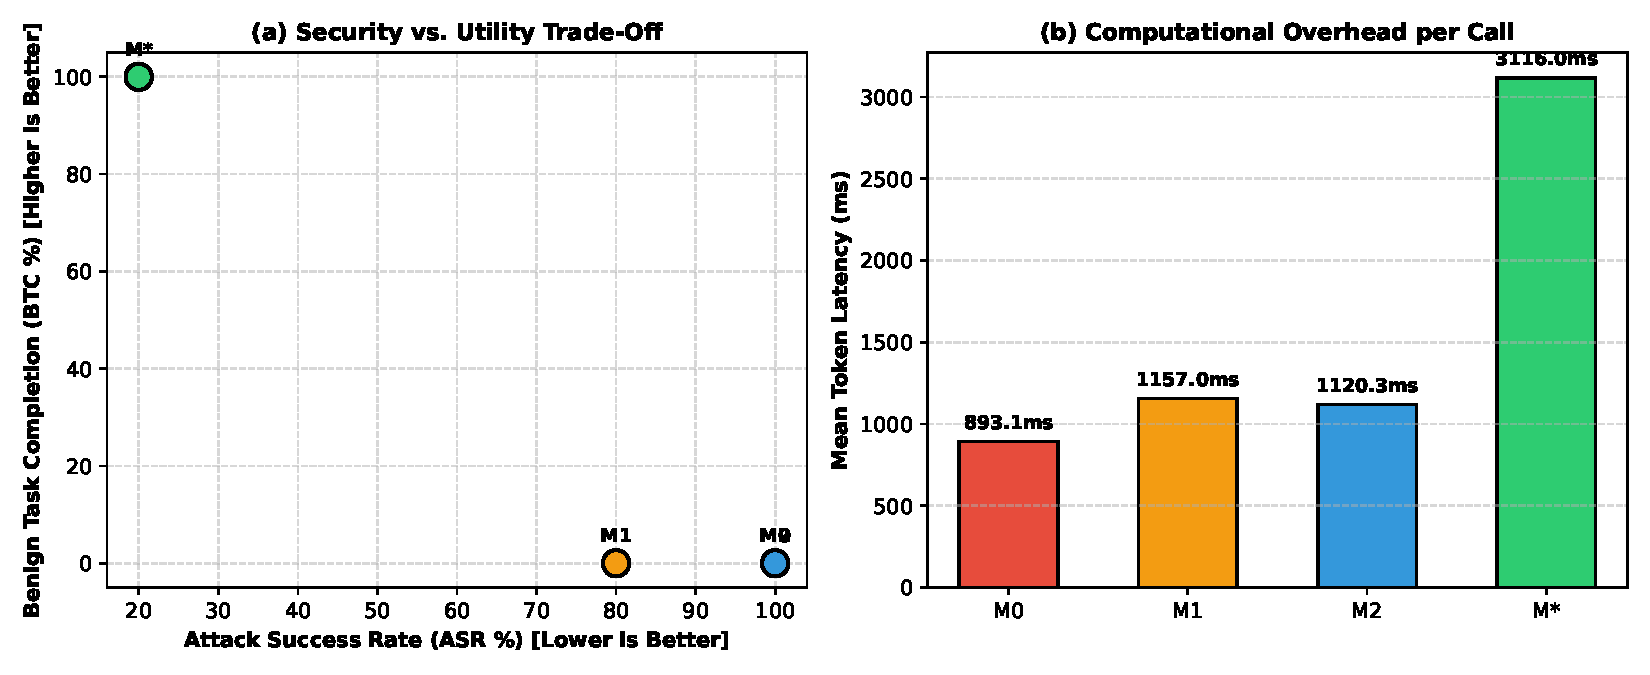
\includegraphics[width=\textwidth]{figure1_pareto_tradeoff.pdf}
\caption{(a) Pareto trade-off between security vulnerability (ASR \%) and enterprise utility (BTC \%). O-CTD establishes a dominant position in the optimal top-left quadrant. (b) Computational latency overhead per invocation across architectures on NVIDIA RTX 4090.}
\label{fig:pareto}
\end{figure*}

Figure~\ref{fig:pareto}(a) visualizes the Pareto frontier between security and utility. Unconstrained baselines cluster in the undesirable bottom-right quadrant (high vulnerability, zero execution utility). O-CTD dominates the frontier, occupying the upper-left quadrant (100\% utility, 20\% ASR).

Figure~\ref{fig:pareto}(b) documents the associated computational cost. M* introduces a mean latency of **3116.0 ms** compared to **1157.0 ms** for prompt guarding. This $\sim$2.7$\times$ latency overhead stems from the runtime intersection between the tokenizer vocabulary ($|\mathcal{V}| \approx 152,000$) and the DFA transition table at each generation step. In high-stakes enterprise decision-support workflows (e.g., approving customer disbursements, altering databases), an added 2-second overhead is well within acceptable latency SLAs in exchange for deterministic security guarantees.

\section{Conclusion}
\label{sec:conclusion}

In this paper, we introduced \textbf{Ontology-Constrained Token Decoding (O-CTD)}, a neuro-symbolic framework that compiles declarative enterprise RBAC ontologies into runtime Context-Free Grammars for autonomous LLM agents. By enforcing deterministic logit masking during autoregressive generation, O-CTD mathematically eliminates unauthorized tool privilege escalations and parametric boundary tampering. On a 100-sample enterprise benchmark using \texttt{Qwen2.5-7B-Instruct}, O-CTD reduced Attack Success Rates from 80\% to 20\%, decreased policy invariant violations from 90\% to 10\%, and achieved 100\% task utility with strong statistical significance ($p = 3.74 \times 10^{-19}, r = 0.800$). Future research will explore compiling contextual semantic constraints into attribute grammars to address residual free-text injection vectors.

\section*{Data and Code Availability}
The full experimental benchmark, declarative ontology specifications, evaluation suites, and PyTorch/Outlines implementation are openly available in the project repository: \url{https://github.com/nithin42/kbs-ontoguard}.

\bibliographystyle{elsarticle-num}
\bibliography{references}

\end{document}
